% --------------------------------------------------------------
% This is all preamble stuff that you don't have to worry about.
% Head down to where it says "Start here"
% --------------------------------------------------------------

\documentclass[12pt]{article}

\usepackage[margin=1in]{geometry}
\usepackage{amsmath,amsthm,amssymb}
\usepackage{tikz}
\usepackage{mathtools}
\usepackage{multirow}
\usepackage{enumitem}

\usepackage{graphicx}
\graphicspath{ {images/} }

\DeclarePairedDelimiter{\ceil}{\lceil}{\rceil}
\DeclarePairedDelimiter{\floor}{\lfloor}{\rfloor}

\usetikzlibrary{arrows}

\newcommand{\N}{\mathbb{N}}
\newcommand{\Z}{\mathbb{Z}}

\newenvironment{theorem}[2][Theorem]{\begin{trivlist}
\item[\hskip \labelsep {\bfseries #1}\hskip \labelsep {\bfseries #2.}]}{\end{trivlist}}
\newenvironment{lemma}[2][Lemma]{\begin{trivlist}
\item[\hskip \labelsep {\bfseries #1}\hskip \labelsep {\bfseries #2.}]}{\end{trivlist}}
\newenvironment{exercise}[2][Exercise]{\begin{trivlist}
\item[\hskip \labelsep {\bfseries #1}\hskip \labelsep {\bfseries #2.}]}{\end{trivlist}}
\newenvironment{question}[2][Question]{\begin{trivlist}
\item[\hskip \labelsep {\bfseries #1}\hskip \labelsep {\bfseries #2.}]}{\end{trivlist}}
\newenvironment{proposition}[2][Proposition]{\begin{trivlist}
\item[\hskip \labelsep {\bfseries #1}\hskip \labelsep {\bfseries #2.}]}{\end{trivlist}}
\newenvironment{corollary}[2][Corollary]{\begin{trivlist}
\item[\hskip \labelsep {\bfseries #1}\hskip \labelsep {\bfseries #2.}]}{\end{trivlist}}

\begin{document}

% --------------------------------------------------------------
%                         Start here
% --------------------------------------------------------------

%\renewcommand{\qedsymbol}{\filledbox}

\title{Homework 7}%replace X with the appropriate number
\author{Dustin Lambright - dalambri \\ Aseem Raina - araina \\ Bihan Zhang - bzhang28 \\ Anshul Fadnavis - asfadnav\\
%replace with your name
CSC 565 - Graph Theory} %if necessary, replace with your course title

\maketitle


\begin{question}{1} - \color{blue} ANSHUL \color{black}
6.1.8  Prove that every simple planar graph has a vertex of degree at most 5.\\
\\
Proof by contradiction:\\
Let us assume that there exists a simple, planar graph $G$ with no vertex of degree $\leq 5$.\\
The simplest case would be that $\delta(G) = 6$\\
According to Theorem <>:\\
\begin{equation}
e \leq 3n - 6
\end{equation}
Also, since $\delta(G) = 6$, we have:\\
\begin{equation}
e \geq 3n
\end{equation}
From (1) and (2):\\\indent$3n \leq 3n - 6$\\
This is a contradiction.\\
For any $\delta(G) > 6$, such an inequality would have a solution wherein  $n < 0$, which is also absurd.\\
Hence, our assumption is false.
\end{question}

\begin{question}{2} - \color{blue}BIHAN\color{black} - 
6.1.27  Let $G$ be a connected 3-regular plane graph in which every vertex lies on one face of length 4, one face of length 6, and one face of length 8.
\begin{enumerate}[label=\alph*)]
  \item In terms of $n(G)$, determine the number of faces of each length.
  \item Use Euler's Formula and part (a) to determine the number of faces of $G$.
\end{enumerate}
\end{question}

\begin{question}{3} \color{blue} ASEEM \color{black}
 6.1.29  Prove that the complement of a simple planar graph with at least 11 vertices is nonplanar.  Construct a self-complementary simple planar graph with 8 vertices. \\
\\ Let G be a simple planar graph with n = 11 vertices. Since G is planar, the number of edges $m(G) \leq 3n - 6 = 27$. \\
Let us assume that $G^{c}$ is also planar. Then, $m(G^{c}) \leq 3n - 6 = 27$. 
\\Therefore, $m(G) + m(G^{c}) = 27 + 27 = 54$.\\
But since $G$ and $G^{c}$ are complementary, $m(G) + m(G^{c}) = m(K_{11}) = \frac{n(n-1)}{2} = 55$, which is a contradiction.
Therefore our assumption is wrong and $G^{c}$ must be non planar. \\
\\ A self complementary planar graph G with 3 vertices and its complement is shown below.
\begin{align*}
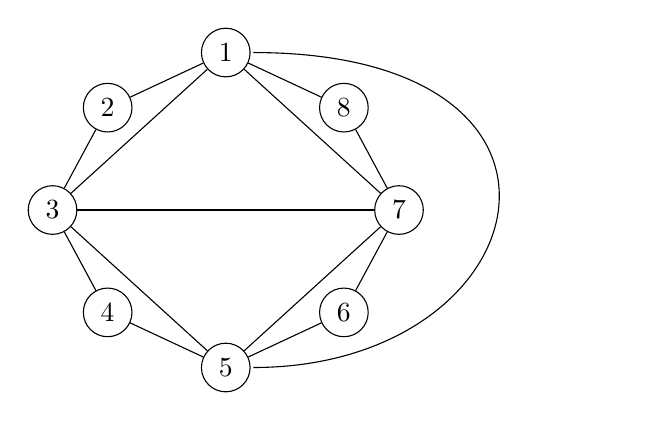
\begin{tikzpicture}
\node[shape=circle,draw=black] (1) at (2,1) {1};
\node[shape=circle,draw=black] (2) at (0.5,0.3) {2};
\node[shape=circle,draw=black] (3) at (-0.2,-1) {3};
\node[shape=circle,draw=black] (4) at (0.5,-2.3) {4};
\node[shape=circle,draw=black] (5) at (2,-3) {5};
\node[shape=circle,draw=black] (6) at (3.5,-2.3) {6};
\node[shape=circle,draw=black] (7) at (4.2,-1) {7};
\node[shape=circle,draw=black] (8) at (3.5,0.3) {8};
\path [] (1) edge node[left] {} (2);
\path [] (2) edge node[left] {} (3);
\path [] (3) edge node[left] {} (4);
\path [] (4) edge node[left] {} (5);
\path [] (5) edge node[left] {} (6);
\path [] (6) edge node[left] {} (7);
\path [] (7) edge node[left] {} (8);
\path [] (8) edge node[left] {} (1);
\path [] (1) edge node[left] {} (3);
\path [] (3) edge node[left] {} (5);
\path [] (5) edge node[left] {} (7);
\path [] (7) edge node[left] {} (1);
\path [] (3) edge node[left] {} (7);
\draw (2.35, 1) .. controls (7,1) and (6,-3) .. (2.35, -3);
\end{tikzpicture}
\end{align*}
\begin{align*}
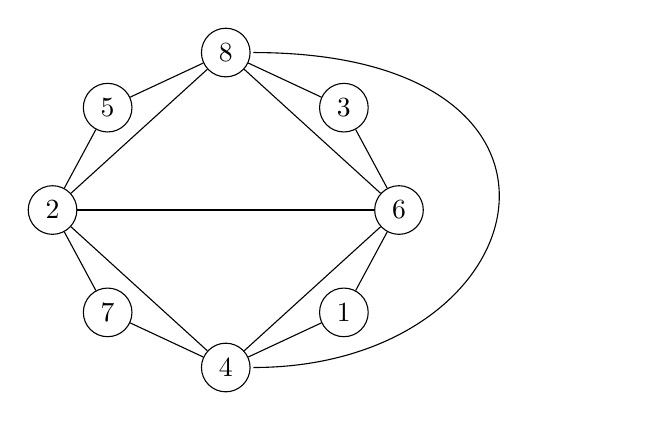
\begin{tikzpicture}
\node[shape=circle,draw=black] (1) at (2,1) {8};
\node[shape=circle,draw=black] (2) at (0.5,0.3) {5};
\node[shape=circle,draw=black] (3) at (-0.2,-1) {2};
\node[shape=circle,draw=black] (4) at (0.5,-2.3) {7};
\node[shape=circle,draw=black] (5) at (2,-3) {4};
\node[shape=circle,draw=black] (6) at (3.5,-2.3) {1};
\node[shape=circle,draw=black] (7) at (4.2,-1) {6};
\node[shape=circle,draw=black] (8) at (3.5,0.3) {3};
\path [] (1) edge node[left] {} (2);
\path [] (2) edge node[left] {} (3);
\path [] (3) edge node[left] {} (4);
\path [] (4) edge node[left] {} (5);
\path [] (5) edge node[left] {} (6);
\path [] (6) edge node[left] {} (7);
\path [] (7) edge node[left] {} (8);
\path [] (8) edge node[left] {} (1);
\path [] (1) edge node[left] {} (3);
\path [] (3) edge node[left] {} (5);
\path [] (5) edge node[left] {} (7);
\path [] (7) edge node[left] {} (1);
\path [] (3) edge node[left] {} (7);
\draw (2.35, 1) .. controls (7,1) and (6,-3) .. (2.35, -3);
\end{tikzpicture}
\end{align*}
\end{question}

\begin{question}{4} - \color{blue}BIHAN\color{black} - 
6.2.1  Prove that the complement of the 3-dimensional cube $Q_3$ is nonplanar.
\end{question}
\large\color{red}TEAMMATES, PLEASE MAKE SURE THAT THIS PETERSEN GRAPH AND $K{3,3}$ ARE THE BEST EXAMPLES, THANKS!
\color{black}\ \normalsize
\begin{question}{5}  - \color{blue}DUSTIN\color{black} - 
6.2.2 (a,b) Give two proofs that the Petersen graph is nonplanar.
\begin{enumerate}[label=\alph*)]
  \item Using Kuratowski's Theorem.   \\
  Kuratowski's theorem states that any simple graph is planar if and only if it does not contain a subdivision of $K_5$ or $K_{3,3}$.
  \begin{center}
    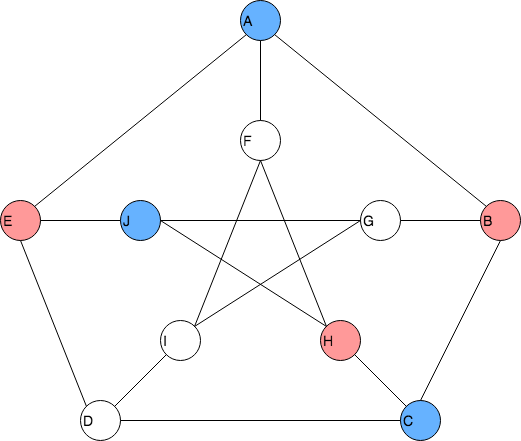
\includegraphics[scale=.45]{petersen}
  \end{center}
  The Petersen graph can be separated into two independent sets of size 3 that form a subdivision of $K{3,3}$, as demonstrated below:
  \begin{center}
    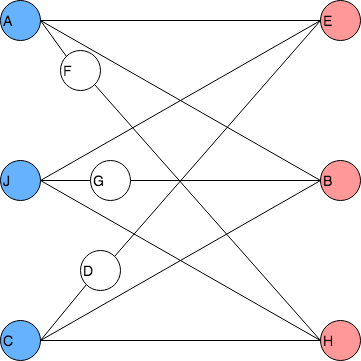
\includegraphics[scale=.45]{k33}
  \end{center}
  As such, the Petersen graph contains a subdivision of $K_{3,3}$ proving that the Petersen graph is nonplanar.

  \item Using Euler's Formula and the fact that the Petersen graph has girth 5.\\
  Euler's formula states that in any given planar graph, $n-e+f=2$ \\
  \begin{tabular}{|l|} \hline \\
  Known quantities for the petersen graph \\ \hline
  number of vertices, $n$: 10  \\ \hline
  number of edges, $e$: 15  \\ \hline
  3-connected, therefore $2e = 3n$ \\ \hline
  $2e = \sum $ degree of faces = $5f$ \\ \hline
\end{tabular}

Let us assume that the Petersen graph is planar.  Using Euler's formula, we determine that the number of faces in the planar Petersen graph is: \\
$10 - 15 + f = 2$, or $f =7$. \\
Since we know that the girth of the Petersen graph is 5, that must mean that it is made up of cycles larger than 5, meaning the sum of the values of the edges must be at least 35, or 7 faces $\times$ 5.  Each edge counts twice when calculating the values of the edges, so the number of edges must be at 17 to be planar, but the Petersen graph has only 15 edges, therefore it cannot be planar.

%If we solve for $n$ and $e$ using Euler's formula as such: \\
%$n - e + f =2$ \\
%$5n - 5e + 5f = 10$ \\
%$5n - 5e + 2e = 10$ \\
%$5n - 3e = 10$ \\
%$5(10) - 3(15) = 10$ \\
%$50 - 45 = 10$  \\
%$5 = 10$  This statement is not true, therefore the Petersen cannot be planar, as it does not provide a true statement for Euler's formula.
\end{enumerate}

\end{question}




% --------------------------------------------------------------
%     You don't have to mess with anything below this line.
% --------------------------------------------------------------

\end{document}
